\chapter{Model framework and results}\label{ch:ensemble} 
In this chapter, we focus on describing the framework of our models that apply ensemble method.  First, let us review some aspects of limit order books. 
\section{Review of limit order books}
According to \cite{rocsu2009dynamic},the electronic limit order books prevail in the world's financial market. A lot of company use electronic trading to promote transactions. An order $x$ with volume $\omega_x<0$($\omega_x>0$,on the other hand) and price $p_x$ is a duty by its owner to buy (sell,on the other hand) up to $|\omega_x|$ units of the security at a price no greater than (no less than, on the other hand) $p_x$. Orders can match the requirements of the other side when arrive are deemed as market order. Orders can not match the requirements of the other side when arrive are called  limit order. The bid price $b_t$ is the leading price among buy orders at time $t$. The ask price $a_t$ is the cheapest price among the prices that all the active sellers are willing to take for. The difference between $a_t$ and $b_t$ is called bid-ask spread. The mean of $a_t$ and $b_t$ is named as mid price. For the limit order book, each time the ask price will be higher than the bid price, since they can not meet the execution requirements mutually. Figure \ref{fig:order_snapshot} shows a snapshot of a 10-level limit order book. The green arrow shows the mid-price between best bid and best ask price. Besides all the ask prices are higher than all the bid prices. If the price of a new coming sell order (respectively, buy order) is lower(respectively, higher) than the best ask(respectively, bid) price, then the order will be executed, otherwise, it will come into the team of limit order books.

\begin{figure}[hbtp]
  \begin{center}
    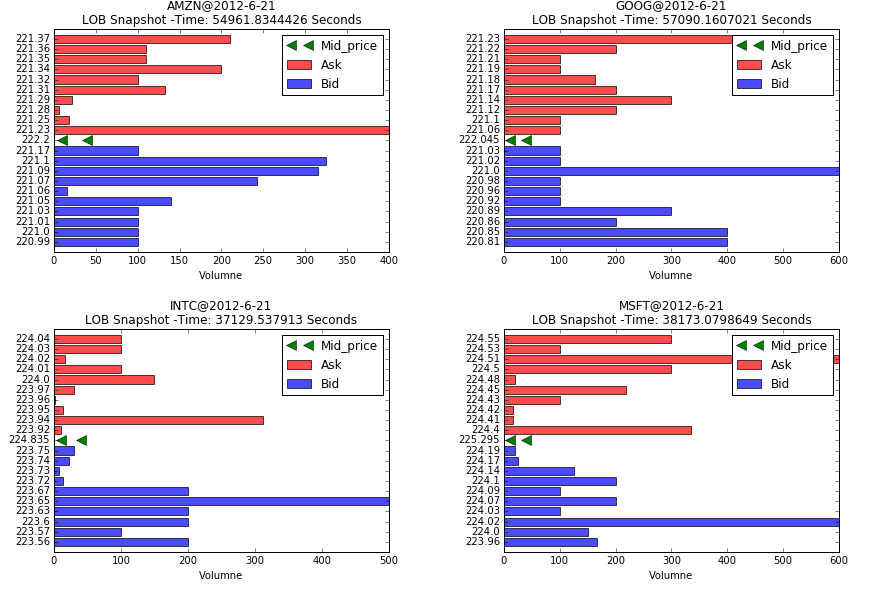
\includegraphics[width=4.5in,height=3.5in]{figures/snapshot.png}
  \end{center}
\caption{Limit order book examples, $x$ axis denotes the volume of each order book and the $y$ axis is the price level of each order book,the left top is AMZN, the right top is GOOG, the left bottom is INTC, and the right bottom is MSFT.Those are snapshots from 2012-06-21} \label{fig:order_snapshot}
\end{figure}

\section{Data description}

In this section, we gibe a detailed description of our dataset which is used to training the models. Our empirical calculations are based on a data set that describes the LOB dynamics for 5 highly liquid stocks traded on Nasdaq during the six-month period of 1 March 2015 to 1 September 2015. 3 The data
that we study originates from the LOBSTER database \cite{huang2015simulating}, which lists all market order arrivals, limit order arrivals, and cancellations that occur on the Nasdaq platform during 09:30 – 16:00 on each trading day. Trading does not occur on weekends or public holidays, so we exclude these days from our analysis. We also exclude market activity during the first and last 1000 seconds of each trading day, to remove any abnormal trading behavior that can occur shortly after the opening auction or shortly before the closing auction. On the Nasdaq platform, each stock is traded in a separate LOB with price–time priority, with a tick size of π = \$0.01. Although this tick size is the same for all stocks on the platform, the prices of
different stocks vary across several orders of magnitude (from about \$1 to more than \$1000). Therefore, the
relative tick size (i.e., the ratio between the stock price and π) similarly varies considerably across different stocks.
To choose the stocks in our sample, we first create a list of all stocks whose mid price remained below\$50.00 during the sample period of 1 March 2015 to 1 September 2015. We then order these stocks according
to their total dollar trade value during this period, and select the first 5 stocks on this list. In descending
order of their levels of market activity, these stocks are Apple (AAPL), Amazon (AMZN), Google (GOOG),Microsoft (MSFT), and  Intel(INTC). Table 1 lists summary statistics describing trading activity
for these 5 stocks during our sample period.
\begin{table}
	\caption{Limit order book statistics}
	\label{sonnets}
	\begin{center}
		\begin{tabular}{|l|c|c|c|c|c|}
			\hline
			 & AAPL & AMZN & GOOG & INTC & MSFT\\[5pt]
			 \hline
		Total number of events at the best quotes& 400391 & 269748 & 147916 & 624040 & 668765 \\[5pt]
			Percentage of market order arrivals & 1.7\% & 2.2\% & 2.4\% & 3.3\% & 1.9\% \\[5pt]
		Percentage of limit order arrivals& 52.9\% & 53.1\% & 52.7\% & 52.9\%& 51.7\%\\[5pt]
			Percentage of limit order cancellations & 45.4\% & 44.7\% & 44.9\% & 43.8\% & 46.4\%\\
			\hline 
		\end{tabular}
	\end{center}
\end{table}
 Extracting information from the ITCH flow and without relying on third-
 party data providers, we analyze stocks from different industry sectors for ten
 full days of ultra-high-frequency intra-day data. The data provides information regarding trades against hidden orders. Coherently, the non-displayable
 hidden portions of the total volume of a so-called iceberg order is not accessible from data. Our ITCH feed data is day-specific and market-wide
 which means that we deal with one file per day with data over all the securities. Information (block A in Figure 1) regarding (i) messages for order
 submissions, (ii) trades and (iii) cancellations is included. For each order,
 its type (buy/sell), price, quantity, and exact time stamp on millisecond ba-
 sis is available. In addition, (iv) administrative messages (i.e. trading halts
 or basic security data), (v) event controls (i.e. start and ending of trading
 days, states of market segments) and (vi) net order imbalance indicator are
 included.
\subsection{Limit order and Message order}
Message and limit order books are processed for each of the 10 days of the
five stocks. More specifically, there are two types of messages particularly
relevant for us: (i) “add order messages”, corresponding to order submissions
and (ii) “modify order messages”, corresponding to updates on the status of
existing orders through order cancellations and order executions. Example
message and limit order books are illustrated in Tables \ref{tab:message} and 3, respectively.
\begin{table}
	\caption{Message book example, a sample on 2012-06-12}
	\label{tab:message}
	\begin{center} 
		\begin{tabular}{|l|c|c|c|c|c|}
			\hline
			Timestamp & ID  & Price & Quantity & Event & Side\\[5pt]
			 \hline
		1275386347944& 6505727 &  126200& 400& 1 & 1\\
		1275386347981& 6505741& 126500& 300& 2 & 1\\
		1275386347981&	6505741&	126500& 300 & 1&-1\\
		1275386348070& 6511439& 126100& 17& 1 & 1 \\
		1275386348070& 6511439& 126100& 17& 3 & 1\\
		1275386348101& 6511469& 126600& 300 & 1 &-1\\
			\hline 
		\end{tabular}
	\end{center}
\end{table}
 
 \begin{table}
 	\caption{Message book event type, a sample on 2012-06-21}
 	\label{tab:type}
 	\begin{center} 
 		\begin{tabular}{|c|c|}
 			\hline
 			Type & Description\\
 			\hline
 			1 & Submission of a new limit order\\
 			2 & Cancellation(Partial deletion)\\
 			3& Deletion (Total deletion of a limit order)\\
 			4 & Execution of a visible limit order \\
 			5 & Execution of a hidden limit order\\
 			\hline 
 		\end{tabular}
 	\end{center}
 \end{table}
  
   \begin{table}
   	\caption{message book direction, a sample on 2012-06-21}
   	\label{tab:direction}
   	\begin{center} 
   		\begin{tabular}{|c|c|}
   			\hline
   			Direction& Description\\
   			\hline
   			-1 & Sell limit order\\
   			1 & Buy limit order\\
   		
   			\hline 
   		\end{tabular}
   	\end{center}
   \end{table}
   
In our data, timestamps are expressed in milliseconds since 1-Jan-1970
and shifted by three hours with respect to Eastern European Time (in the
data the trading day goes from 7:00 to 15:25). ITHC feed prices are recorded
with a 4 decimal digits precision and in our data decimal point is removed by
multiplying the price by 10.000. Currency is in Euro for Helsinki exchange.
The tick size, defined as the smallest possible gap between the ask and bid
prices, is one cent. Similarly, orders’ quantities are constrained to integers
greater than one. An example of our LOB is the following:

\begin{table}
   	\caption{limit book direction, a sample on 2012-06-12}
   	\label{tab:limit}
   	\begin{center} 
   		\begin{tabular}{c c c c c c c c c}
   			\hline
   			\multicolumn{4}{c}{ Level 1} & \multicolumn{4}{c}{Level 2}&... \\
   			\hline
   			 \multicolumn{2}{c}{Ask}  & \multicolumn{2}{c}{Bid} & \multicolumn{2}{c}{Ask}  & \multicolumn{2}{c}{Bid}&... \\
   			 \hline
   			  Price & Quantity & Price& Quantity& Price& Quantity& Price & Quantity\\
   			  126300& 300 & 126100& 17& 126400& 4765& 126000& 2800&...\\
   			  126300& 300& 126100& 17& 126400& 4765& 126000& 2800&...\\
   			  126300& 300& 126100& 17& 126400& 4765& 126000& 2800&...\\
   			  126111& 291& 126000& 2800& 126200& 300& 125900& 1120&...\\
   			  126100& 291& 126000& 2800& 126200& 300& 125900& 1120&...\\
   			  126100& 291& 126000& 2800& 126200& 300& 125900& 1120&...\\
   		
   			\hline 
   		\end{tabular}
   	\end{center}
\end{table} 

\subsection{Features}
We follow an event based inflow, as has been used in [31]. This is due to
that events (i.e. orders, executions and cancellations) do not follow a uniform
inflow rate. Time intervals between two consecutive events can vary from
milliseconds to several minutes of difference. Event based data representation
avoids issues related to such big differences in data flow. As a result, each of
our representations is a vector that contains information for 10 consecutive
events. Event based data description leads to a dataset of approximately
half a million representations (i.e. 394337 representations). We represent
these events using the 144-dimensional representation proposed recently by
Kercheval and Zhang [28], formed by three types of features: a) the raw
data of a ten-level limit order containing price and volume values for bid
and ask orders, b) features describing the state of the LOB exploiting past
information and c) features describing the information edge in the raw data
by taking time into account. Derivation of time, stock price and volume are
calculated for short and long term projection. Particularly, types in features
u 7 , u 8 and u 9 are: trades, orders, cancellations, deletion, execution of a visible
limit order and execution of a hidden limit order respectively. The features are listed in the following figure and can be referred in \cite{kercheval2015modelling}  
\begin{figure}[hbtp]
  \begin{center}
    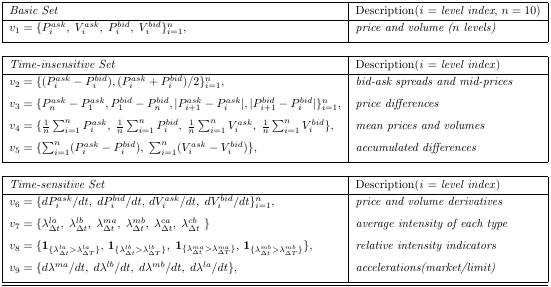
\includegraphics[width=4.5in,height=3.5in]{figures/features.png}
  \end{center}
\caption{Features to build models} \label{fig:feature}
\end{figure}


\subsection{Order price,order book volume, and order book type}
Here we study some properties of order price,order book volume, and order book type in a given day.
\begin{figure}[hbtp]
  \begin{center}
    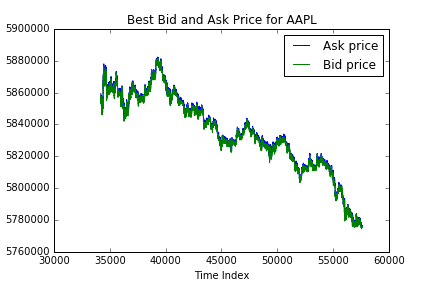
\includegraphics[width=3in,height=2.5in]{figures/AAPL_price.png}
  \end{center}
\caption{Best bid and ask price of AAPL in 2012-06-21} \label{fig:aapl_price}
\end{figure}
\begin{figure}[hbtp]
  \begin{center}
    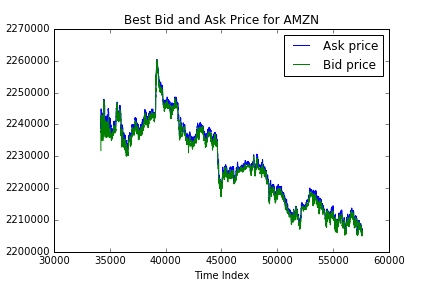
\includegraphics[width=3in,height=2.5in]{figures/AMZN_price.png}
  \end{center}
\caption{Best bid and ask price of AMZN in 2012-06-21} \label{fig:amzn_price}
\end{figure}

\begin{figure}[hbtp]
  \begin{center}
    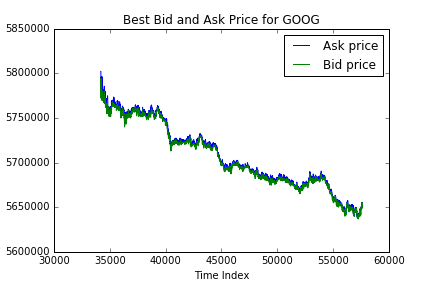
\includegraphics[width=3in,height=2.5in]{figures/GOOG_price.png}
  \end{center}
\caption{Best bid and ask price of GOOG in 2012-06-21} \label{fig:goog_price}
\end{figure}

\begin{figure}[hbtp]
  \begin{center}
    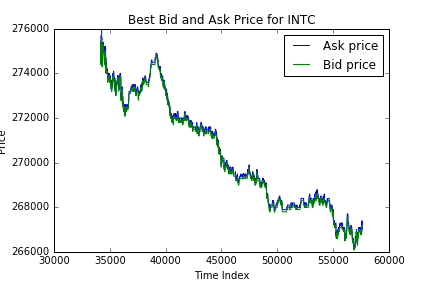
\includegraphics[width=3in,height=2.5in]{figures/INTC_price.png}
  \end{center}
\caption{Best bid and ask price of INTC in 2012-06-21} \label{fig:intc_price}
\end{figure}

\begin{figure}[hbtp]
  \begin{center}
    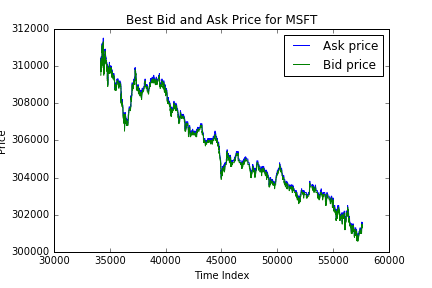
\includegraphics[width=3in,height=2.5in]{figures/MSFT_price.png}
  \end{center}
\caption{Best bid and ask price of MSFT in 2012-06-21} \label{fig:msft_price}
\end{figure}

We can see from figure \ref{fig:aapl_price} to figure \ref{fig:msft_price}, both best ask price and best bid price are decreasing in the given day. \\

\begin{figure}[hbtp]
  \begin{center}
    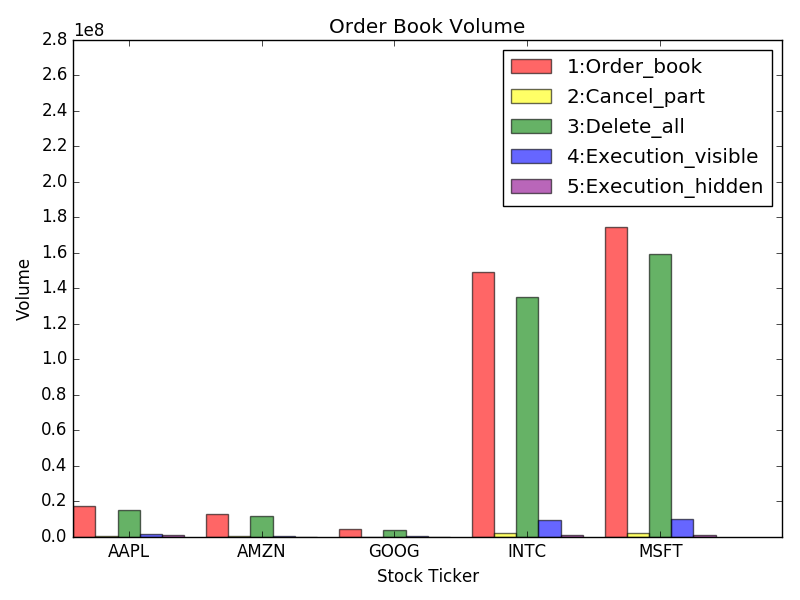
\includegraphics[width=4in,height=4in]{figures/order_book_volume.png}
  \end{center}
\caption{Order book volume comparison for five stocks in 2012-06-21} \label{fig:order_book_volume}
\end{figure}

From figure\ref{fig:order_book_volume} we can see that for all the five stocks, among all the types, putting a new order book and cancel all the order book accounting for the vast majority of the proportion. In chapter 1, we have mentioned that a momentum strategy will put and cancel order book in a very short time to ignite the momentum from which the executor can beneficial from the spread by other investors. 

\begin{figure}[hbtp]
  \begin{center}
    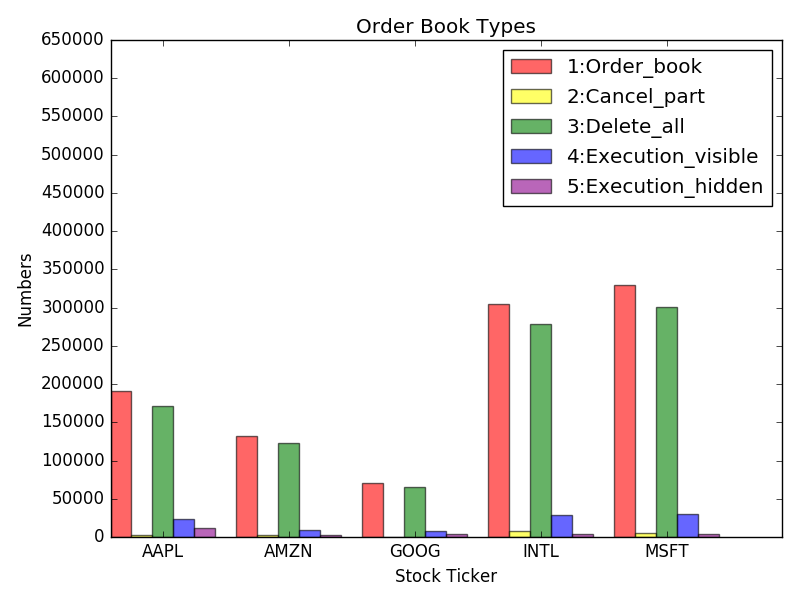
\includegraphics[width=4in,height=4in]{figures/order_book_type.png}
  \end{center}
\caption{Order book type comparison for five stocks in 2012-06-21} \label{fig:order_book_type}
\end{figure}
Figure\ref{fig:order_book_type} shows the same trend with the situation of order book volume. It is another example to show the arbitrage strategy of high frequency trading companies.


\begin{figure}[hbtp]
  \begin{center}
    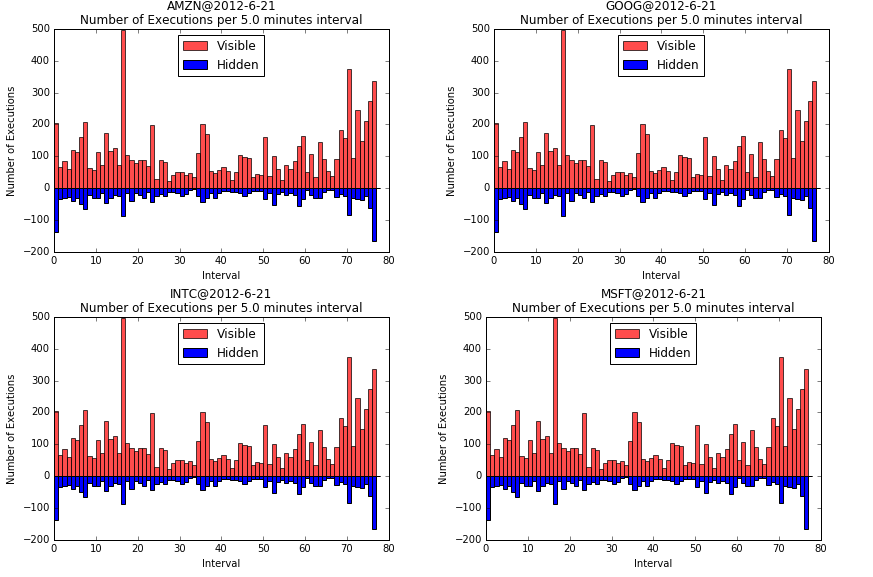
\includegraphics[width=6in,height=5in]{figures/execution.png}
  \end{center}
\caption{Number of trading in 2012-06-21,$x$ axis is the time interval and $y$ axis is the number of executions. Each band in time interval represents 5 minutes.The top left panel shows the result of AMZN, the top right panel shows the result of GOOG,the bottom left panel shows the result of INTC, and the bottom right panel shows the result of MSFT.   } \label{fig:execution}
\end{figure}

\begin{figure}[hbtp]
  \begin{center}
    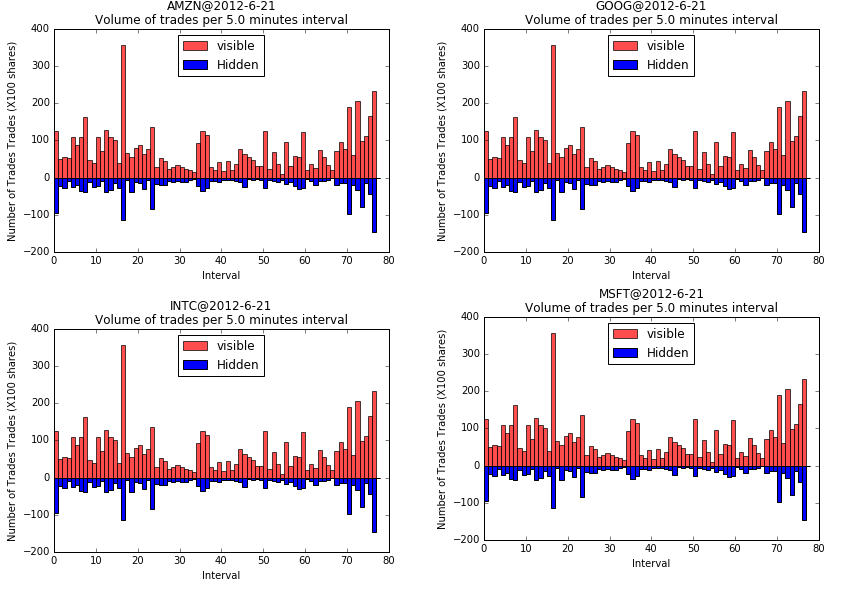
\includegraphics[width=6in,height=5in]{figures/volume_trade.png}
  \end{center}
\caption{Volume of trading in 2012-06-21,$x$ axis is the time interval and $y$ axis is the number of executions. Each band in time interval represents 5 minutes.The top left panel shows the result of AMZN, the top right panel shows the result of GOOG,the bottom left panel shows the result of INTC, and the bottom right panel shows the result of MSFT.  } \label{fig:volume_trade}
\end{figure}

\begin{figure}[hbtp]
  \begin{center}
    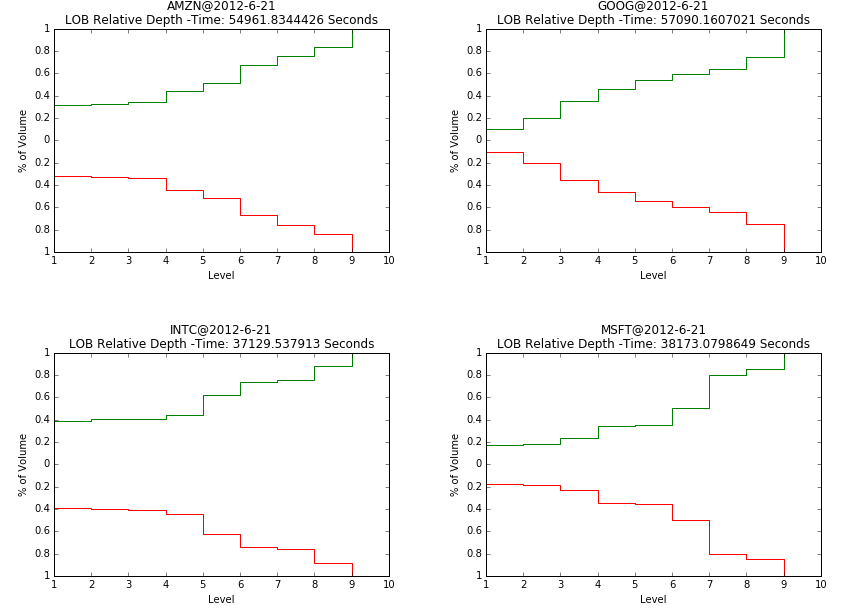
\includegraphics[width=6in,height=5in]{figures/depth.png}
  \end{center}
\caption{Relative depth in 2012-06-21,$x$ axis is the price level and $y$ axis is the percentage of total volume. The top left panel shows the result of AMZN, the top right panel shows the result of GOOG,the bottom left panel shows the result of INTC, and the bottom right panel shows the result of MSFT. . } \label{fig:depth}
\end{figure}

\section{Model framework}
Our model aims to predict the arbitrage opportunities of limit order book price change. there are two kinds of arbitrage in our case: ask price lower arbitrage and bid price higher arbitrage. We know that in any given time, the ask price will always higher than the bid price, so there is no arbitrage. However if the ask price at future $\Delta t$ time is lower than the current price now, then there exists the arbitrage. How to realize it? The arbitrageur can sell short the stock at current bid price $b_t $ and wait for $\Delta t$ time, buy the stock from market with the price of ask price $a_{t+\Delta t}$, to return the stock required by the short positions, the spread he can earn without risk is $b_t-a_{t+\Delta t}$. On the bid high situation, the arbitrage strategy is similar. Figure \ref{fig:ask_low},figure \ref{fig:bid_high},and figure\ref{fig:no_arbi} give us examples of ask low arbitrage, bid high arbitrage, and no arbitrage case respectively.

\begin{figure}[hbtp]
  \begin{center}
    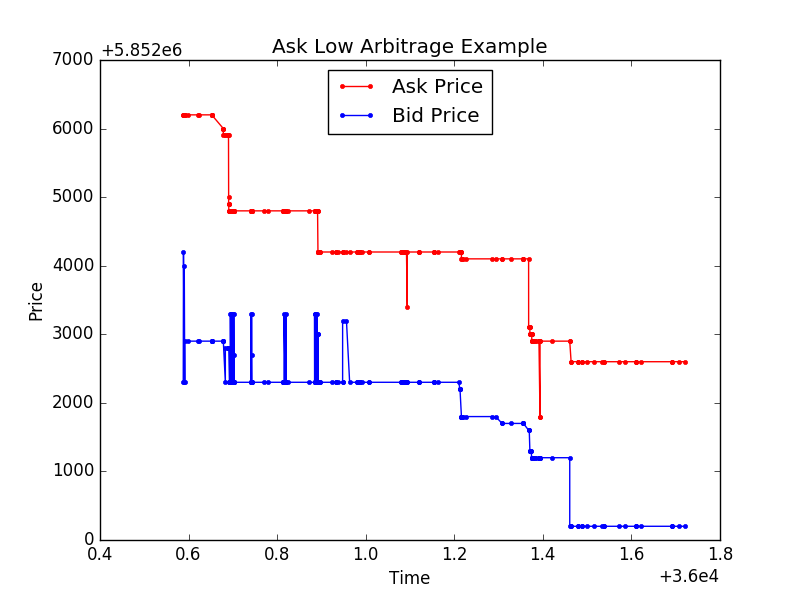
\includegraphics[width=4in,height=4in]{figures/ask_low_example.png}
  \end{center}
\caption{Ask low arbitrage example} \label{fig:ask_low}
\end{figure}


\begin{figure}[hbtp]
  \begin{center}
    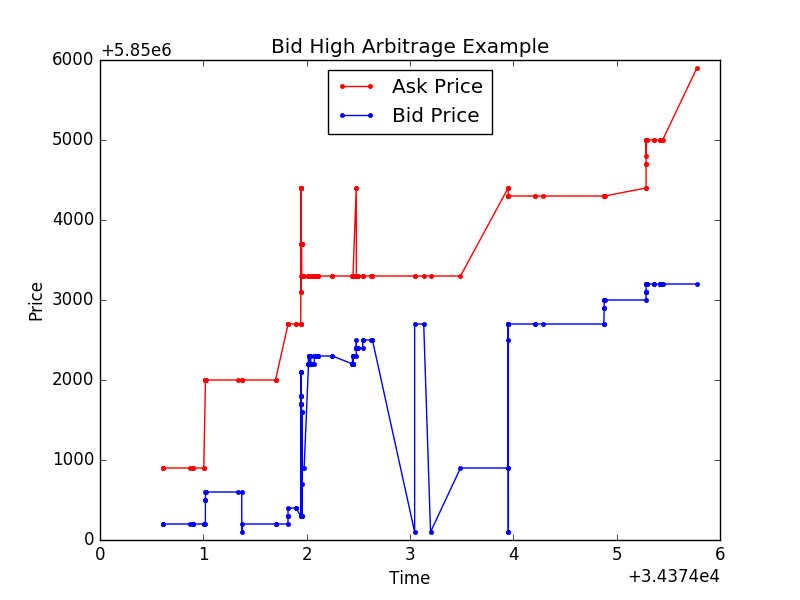
\includegraphics[width=4in,height=4in]{figures/bid_high_example.png}
  \end{center}
\caption{Bid high arbitrage example} \label{fig:bid_high}
\end{figure}


\begin{figure}[hbtp]
  \begin{center}
    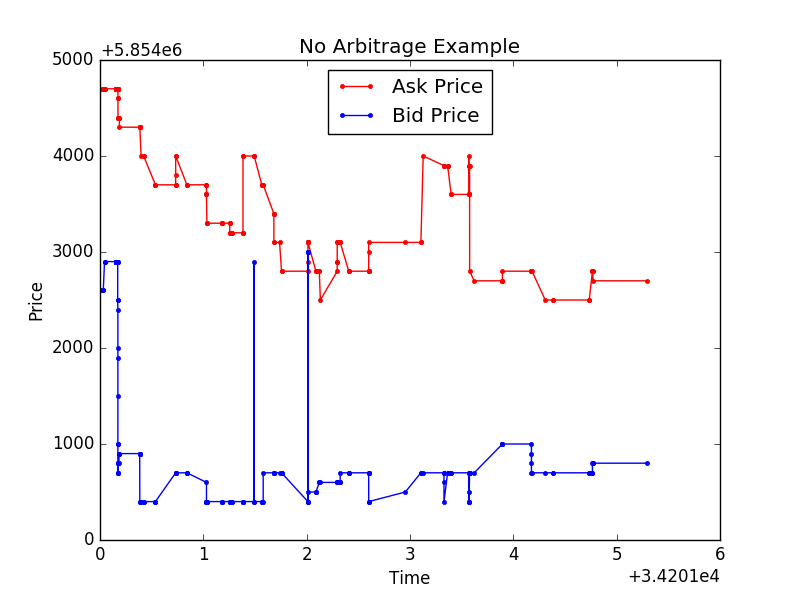
\includegraphics[width=4in,height=4in]{figures/no_arbi_example.png}
  \end{center}
\caption{No arbitrage example} \label{fig:no_arbi}
\end{figure}

Instead of predicting the price change of future events, like most past papers did, we focus on predict the price change in a fixed future time interval,e.g. 5 seconds later.

\begin{figure}[hbtp]
  \begin{center}
    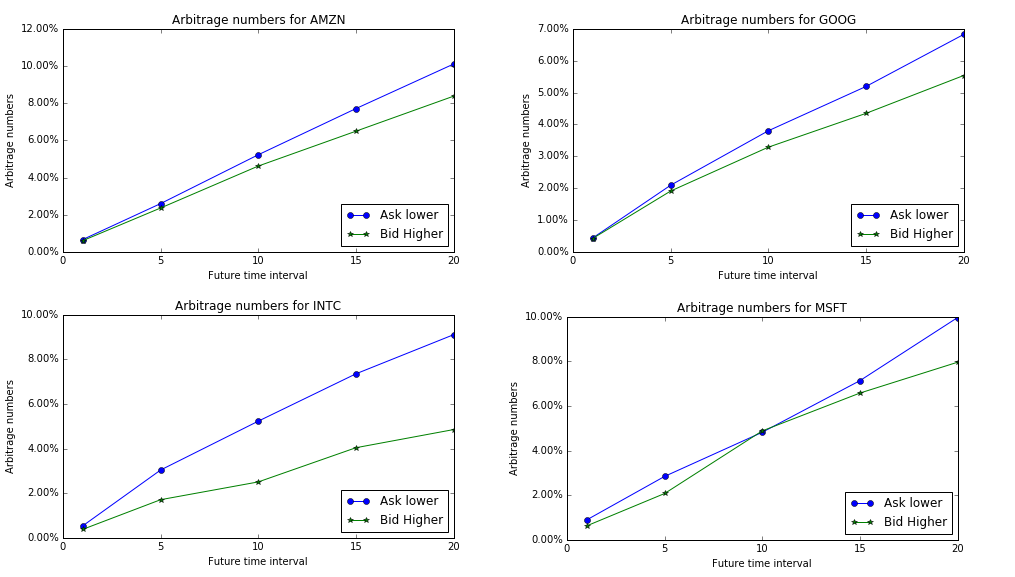
\includegraphics[width=4in,height=4in]{figures/arbitrage_time.png}
  \end{center}
\caption{Arbitrage numbers based on future time interval} \label{fig:arbitrage_time}
\end{figure}

From figure \ref{fig:arbitrage_time}, we can find that the arbitrage numbers for both bid-high and ask-low opportunities are increasing. For the five seconds time interval, the percentage of arbitrage opportunities among all the transaction is around 2\% for each stock listed in the figure. For the ten seconds time interval, the arbitrage percentage increases to around 4\%, which almost doubled. 

Generally speaking, separate learning models should be built for different metrics
depicting limit order book dynamics. To build a machine learning model for a specific
metric, the following four-phase process is employed.
• Features representation: the data in the order book and message book is
converted into a format suitable for machine learning methods to manipulate.
• Learning model construction: Models of Adaboost and random forest 
• Learning model validation: the model is evaluated and validated using particular performance measurements.
• Unseen-data classification: the constructed learning model automates the
forecasting of the chosen metric in real time.


\section{Model measurement and numerical results}
As we mentioned before, the arbitrage opportunities are rare events among all the placement of order books. For example, the percentages of arbitrage opportunities of five seconds interval is only around 2 \%, so the accuracy rate of model is not a good measurement, because if we define all the results of testing sample as no arbitrage, we can still get a very high accuracy rate, which is around 98 \%. Therefore we introduce precision, recall and f1 score to deal with this problem. \\
Some terms here:\\
Positive (P): Observation is positive, in our case, arbitrage opportunity will occur in the future.\\
Negative (N): Observation is negation, in our case means there is no arbitrage in the future. \\
True positive(TP): Observation is positive and is classified as positive, in our case means the detected arbitrage opportunity is real arbitrage opportunity.\\
False negative(FN):Observation is positive but is classified as negative,in our case means the detected arbitrage opportunity is not an arbitrage opportunity\\
True negative(TN):Observation is negative and is classified as negative,in our case means the detected no arbitrage case is actually no arbitrage\\
False positive(FP):Observation is positive but is classified as negative,in our case means the detected arbitrage case is actually no arbitrage. \\
The precision is: \\
\begin{equation}
Precision=\frac{TP}{TP+FP}=\frac{positive\ predicted\ correctly}{all\ positive\ predictions}
\end{equation} 
The recall is:\\
\begin{equation}
Recall=\frac{TP}{TP+FN}=\frac{predicted\ to\ be\ positive}{all\ positive\ observations}
\end{equation} 
F1 score:\\
\begin{equation}
F_1=2\frac{Precision*Recall}{Precision+Recall}
\end{equation} 
Actually, $F1$ score is the harmonic mean of precision and recall\\ 
The following shows the results of predicting ask low opportunity of stock AMZN.

\begin{table}[htp!]
	\caption{AMZN ask-low arbitrage opportunity prediction(5 seconds)}
	\label{ask_low_prediction}
	\begin{center}
		\begin{tabular}{|c|c|c|c|c|c|c|}
			\hline
			 Model& Training & Training  & Test  & Test & Test & Test \\[5pt]
			 & time(s) & F1 score & time(s) & Precision & Recall & F1 score \\[5pt]
			 \hline
			 Logistic regression(Lasso penalty)& 408.0 & 8.1 \% & 0.003 & 6.2\% & 61.5\%& 11.2\%\\[5pt]
			 Logistic regression(Ridge penalty)& 12.1 & 8.0 \% & 0.02 &  6.1\% & 61.5\%& 11.2\%\\[5pt]
			 SVM(Poly 2 kernal,5000 estimator)& 100.4 & 60.6 \% & 4.1 &  33.8\% & 100.0\%& 50.6\%\\[5pt]
			 Decision Tree(no pruning)& 4.0 & 61.2 \% & 0.005 &  37.7\% & 94.2\%& 53.8\%\\[5pt]
			 Adaboost(number of estimate=100)& 277.4 & 99.8 \% & 0.3 & 77.7 \% & 88.6 &  82.8\% \\[5pt]
			 Random forest(number of estimate=100)& 49.0 & 95.6 \% & 0.16 & 73.1 \% & 99.0\% &  84.1\% \\[5pt]		 	
	 		\hline 
		\end{tabular}
	\end{center}
\end{table}
 
Here the training samples are 90000 and test samples are 10000. Computer is 8G memory and Intel Xeon E3. \\

\section{Feature importance}

According toAccording toAccording toAccording toAccording toAccording toAccording toAccording toAccording toAccording toAccording toAccording toAccording toAccording toAccording toAccording toAccording toAccording toAccording toAccording toAccording toAccording toAccording toAccording toAccording toAccording toAccording toAccording toAccording toAccording toAccording toAccording toAccording toAccording toAccording toAccording toAccording toAccording toAccording tov
\begin{table}[htp!]
	\caption{Feature importance based on random forest model}
	\label{feature_importance}
	\begin{center}
	\rotatebox{270}{
		\begin{tabular}{cccccccc}
		\hline
			\multicolumn{2}{c}{ AMZN} & \multicolumn{2}{c}{GOOG}& \multicolumn{2}{c}{INTC}& \multicolumn{2}{c}{MSFT}\\
			\hline
			 Feature index  &  Importance& Feature index  &  Importance &Feature index  &  Importance & Feature index  &  Importance\\
			 \hline
		107& 3.997699& 41& 2.497344& 16& 4.930035& 28& 3.777894\\
		108& 2.531017& 3& 2.077711& 36& 3.584072& 12& 3.668482\\
		116& 1.72645& 51& 1.911522& 40& 3.271213& 16& 3.462065\\
		12& 1.523849& 71& 1.860316& 14& 2.930865& 36& 3.307528\\
		41& 1.489288& 111& 1.7199& 30& 2.830366& 8& 3.134871\\
		52& 1.401763& 70& 1.511696& 20& 2.694488& 26& 2.863927\\
		61& 1.390584& 82& 1.503223& 22& 2.594267& 30& 2.783838\\
		51& 1.296778& 42& 1.476138& 38& 2.575397& 20& 2.782014\\
		1& 1.26687& 7& 1.446197& 28& 2.565284& 24& 2.752804\\
		81& 1.24307& 52& 1.413531& 32& 2.510037& 32& 2.722132\\
		3& 1.240166& 53& 1.410323& 18& 2.485869& 38& 2.660868\\
		9& 1.222178& 80& 1.379994& 24& 2.388528& 81& 2.45301\\
		79& 1.187279& 8& 1.3286& 82& 2.289012& 82& 2.312318\\
		80& 1.168383& 84& 1.316409& 12& 2.165716& 40& 2.276727\\
		53& 1.16105& 24& 1.246773& 26& 2.119569& 34& 2.149401\\
		54& 1.150503& 15& 1.223152& 4& 2.032679& 10& 1.790342\\
		82& 1.150272& 55& 1.214248& 8& 2.007556& 18& 1.765228\\
		118& 1.133169& 16& 1.211959& 34& 1.950585& 14& 1.727172\\
		7& 1.131877& 57& 1.199527& 81& 1.896318& 22& 1.649081\\
		84& 1.099623& 1& 1.178082& 6& 1.697322& 84& 1.515854\\
\hline 
		\end{tabular}
		}
	\end{center}
\end{table}


\begin{figure}[hbtp]
  \begin{center}
    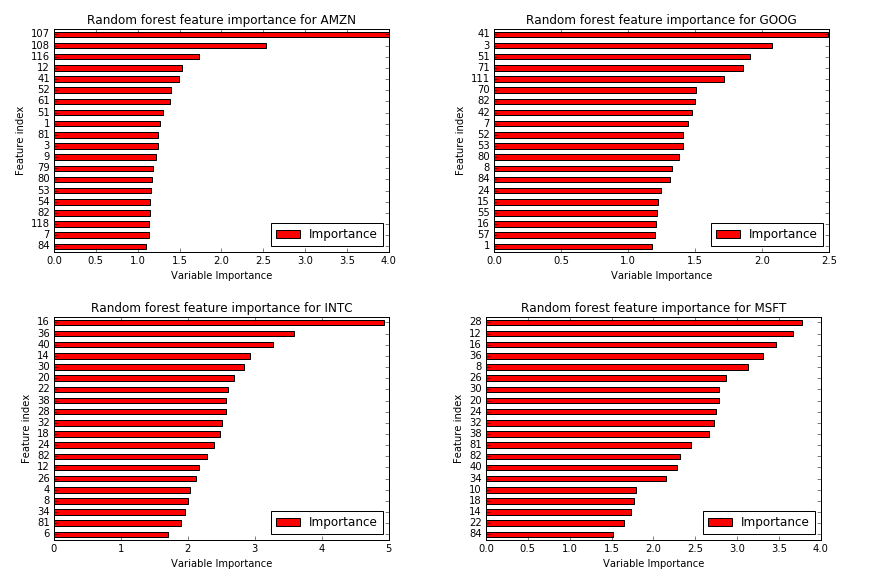
\includegraphics[width=6in,height=5in]{figures/feature_importance.png}
  \end{center}
\caption{Feature importance. $x$ axis is the feature importance and $y$ axis is the corresponding feature index.The top left panel shows the result of AMZN, the top right panel shows the result of GOOG,the bottom left panel shows the result of INTC, and the bottom right panel shows the result of MSFT. } \label{fig:feature_importance}
\end{figure}


\section{Trading strategy}
According to \cite{zhou2015evolution},PnL is the profit and loss through transaction which can be written as follows:\\
\begin{equation}       
PnL=\left\{          
  \begin{array}{ll}   
    y-c  & y>=\alpha, buy\ action   \\  
     -y-c & y<=-\alpha, sell\ short\ action \\
     0 & otherwise
  \end{array}
\right.       
\end{equation}
where y is the net capital gain from transaction, $\alpha$ is significant level and $c$ is the trading cost.In the following we define a simple buy- low and sell high strategy.The details is in algorithm \ref{alg:trading_algorithm}


\begin{algorithm}[H]
\caption{Naive trading algorithm,\cite{breiman1996bagging}}\label{alg:trading_algorithm}

				         		    \nl initialize: PnL=0\\				         		    
				         		    \nl \For{i =1 to length(test\_set)}{
				         		    \nl input test\_set[i] features into model and get result of Predict[i]\\
				         		    \nl \If{Predict[i]==1(Ask low)}{
				         		         Sell short at bid price\\
				         		         Clear the short option $\Delta t$ seconds later\\
				         		         PnL+=$Bid\_price_{t}-Ask\_price_{t+\Delta t}$}
				         		        \ElseIf{Predicted[i]==-1(Bid high)}
				         		         {Buy at ask price\\
				         		         Sell at bid price $\Delta t$ seconds later\\
				         		          PnL+=$Bid\_price_{t+\Delta t}-Ask\_price_t$}\\
				         		        \Else
				         		         {Take no action} \\
				         		    \nl  \Return PnL 
				         		     }				  				         		    
			\end{algorithm} \\			
More vivid to show in the following figure \ref{fig:strategy_algorithm}

\begin{figure}[hbtp]
  \begin{center}
    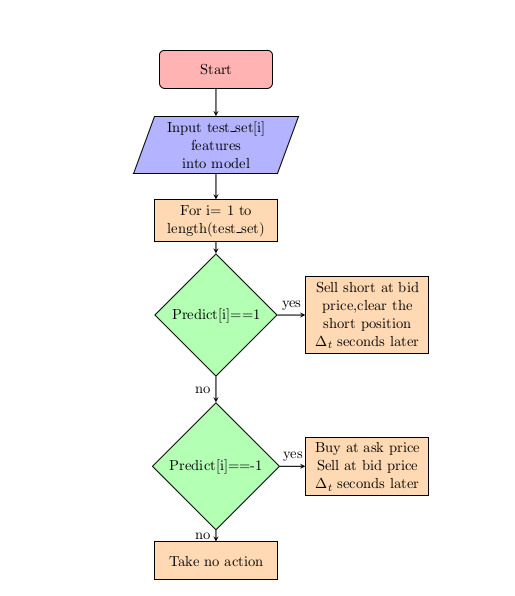
\includegraphics[width=4.5in,height=3.5in]{figures/strategy_algorithm.png}
  \end{center}
\caption{Naive trading strategy framework} \label{fig:strategy_algorithm}
\end{figure}


Figure \ref{fig:arbitrage_plot} gives us an example on how to conduct an arbitrage trading, when the ask-low cases(green triangles) occur, we can sell short at the current bid price and buy the stock back at the future ask price. Similarly, when the bid-high cases (red triangles)occurs, we can buy the stock at the current ask price and sell the stock to the market at the future bid price. 

\begin{figure}[hbtp]
  \begin{center}
    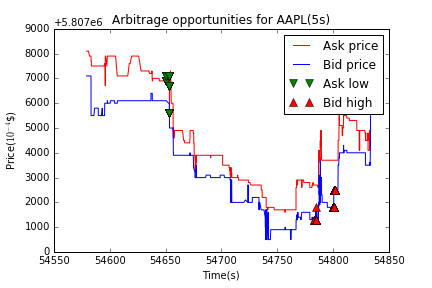
\includegraphics[width=4.5in,height=3.5in]{figures/arbitrage_plot.png}
  \end{center}
\caption{Arbitrage opportunities, x-axis is the time elapsed in second and the y axis is the stock price in US dollar.Blue line is bid price and red line is ask price, the triangles are the places where arbitrages occur, the green triangle is ask-low case and the red triangle is the bid high case. } \label{fig:arbitrage_plot}
\end{figure}


Figure \ref{fig:pnl} shows the PnL for the four stocks. The red dot represents the bid-high cases and the blue dots represent the ask-low cases. If the dot lies above the x axis,it means that this transaction will earn money and vice versa.
\begin{figure}[hbtp]
  \begin{center}
    \includegraphics[width=6in,height=5in]{figures/pnl_total.png}
  \end{center}
\caption{Profit and Loss,  $x$ axis represents the predicted arbitrage index and $y$ axis is profit or loss for each transaction.The top left panel shows the result of AMZN, the top right panel shows the result of GOOG,the bottom left panel shows the result of INTC, and the bottom right panel shows the result of MSFT. } \label{fig:pnl}
\end{figure}

\begin{figure}[hbtp]
  \begin{center}
    \includegraphics[width=6in,height=5in]{figures/cum_pnl_total.png}
  \end{center}
\caption{Cumulated Profit and Loss,  $x$ axis represents the predicted arbitrage index and $y$ axis is profit or loss for each transaction.The top left panel shows the result of AMZN, the top right panel shows the result of GOOG,the bottom left panel shows the result of INTC, and the bottom right panel shows the result of MSFT. } \label{fig:cum_pnl}
\end{figure}
				